\documentclass{report}
\input{preamble}
\input{macros}
\input{letterfonts}

\title{\Huge{Derivate}}
\author{\huge{Francesco Sermi}}
\date{Luglio 2023}

\begin{document}

\maketitle
\newpage% or \cleardoublepage
% \pdfbookmark[<level>]{<title>}{<dest>}
\cleardoublepage
\pdfbookmark[section]{\contentsname}{toc}
\tableofcontents
\pagebreak

\chapter{Introduzione al concetto di derivata e notizie storiche}

All'inizio dell'Ottocento, per la corretta descrizione dei fenomeni fisici come il moto parabolico, bisognava trovare un procedimento matematico \textbf{formale} che consentisse di:
\begin{enumerate}[label=\protect\circled{\arabic*}]
	\item trovare la tangente in un qualsiasi punto $x_0$ appartenente alla funzione;
	\item trovare l'area sotto al grafico di una qualunque curva.
\end{enumerate}
Questi due problemi furono affrontati da numerosi matematici del tempo e fu anche alla base di uno dei più grandi dibattiti della storia della matematica, ovvero quello sull'attribuzione della paternità della branca del calcolo infinitesimale, la quale era stata scoperta, quasi contemporaneamente, dal celebre matematico e fisico Isaac Newton e dal matematico Gottfried Wilhelm von Leibniz, che si concluse con l'attribuzione del titolo di "\emph{padre}" di questa branca a Newton. \\
Ma, adesso, concentriamoci piuttosto sul perché trovare la tangente con una curva qualunque fosse così tanto complesso. Nel caso di una curva polinomiale\footnote{ovvero una curva del tipo $f(x)=a_nx^n + a_{n-1}x^{n-1} + \ldots + a_1x + a_0$} come ad esempio la funzione $f(x) = x^2$:
\begin{align*}
&\begin{cases}
	y = x^2 \\
	y = mx + q
\end{cases}
\text{si impone il passaggio della retta per il punto $P(x_0;f(x_0))$} \implies \\
&\implies \begin{cases}
	y = x^2 \\
	y - f(x_0) = m(x - x_0) \implies y = mx - mx_0 + f(x_0)
\end{cases}
\end{align*}
Possiamo a questo punto definire l'equazione risolvente:
\begin{equation*}
	\begin{cases}
		y = x^2 \\
		y = mx - mx_0 + f(x_0)
	\end{cases}
	\implies x^2 = mx - mx_0 + f(x_0) \implies x^2 - mx + mx_0 - f(x_0) = 0
\end{equation*}
E porre il discriminante $\Delta$ uguale a $0$, per individuare i valori $m$ (ovvero del coefficiente angolare della retta) passanti per il punto $P(x_0; f(x_0))$ tali da determinare un'unica soluzione, quindi un solo punto di intersezione (in quanto la retta è tangente). Nel nostro esempio:
\begin{equation*}
	\Delta = 0 \implies b^2 - 4ac = 0 \implies m^2 - 4(mx_0 - f(x_0) = 0
\end{equation*}
Prendendo una curva non polinomiale, come una funzione trascendentale oppure una funzione esponenziale, non è possibile porre un discriminante:
\begin{equation*}
\begin{cases}
	y = e^x \\
	y = mx - mx_0 + f(x_0)
\end{cases} \nexists \Delta
\end{equation*}
Per trovare la retta tangente in un qualunque punto dobbiamo ragionare in maniera differente da come fatto finora. Innanzitutto, possiamo notare un'interessante proprietà di una retta tangente al punto $P(x_0; f(x_0))$ appartenente alla funzione $f(x)$.
\begin{figure}[H]
	\centering
	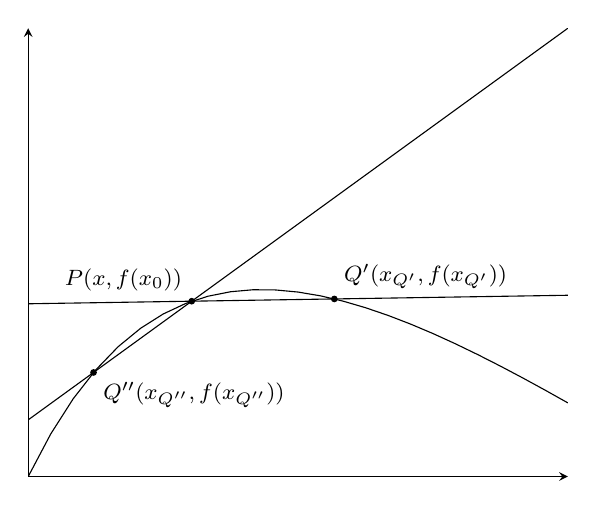
\begin{tikzpicture}
	\begin{axis}[axis lines=left, domain=0.5:1, ticks=none]
		\addplot[]{(ln(x))^(3) - (ln(x))^2 - (ln(x))};
		\node[anchor=north west] at (axis cs:1, 0) {$x$};
		\node[anchor=north east] at (axis cs:0, 1) {$y$};
		\node[anchor=south east, font=\footnotesize] at (axis cs:0.65149157,0.16621364) {$P(x, f(x_0))$};
		\draw[color=black, fill=black] (axis cs:0.65149157,0.16621364) circle[radius=1pt];
		\addplot[]{1.2800065971957*x - 0.6676998645145};
		\node[anchor=south west, font=\footnotesize] at (axis cs:0.7835948738844, 0.169891553757) {$Q'(x_{Q'}, f(x_{Q'}))$};
		\node[anchor=north west, font=\footnotesize] at (axis cs:0.5605041663522, 0.049749166172) {$Q''(x_{Q''}, f(x_{Q''}))$};
		\draw[color=black, fill=black] (axis cs:0.7835948738844, 0.169891553757) circle[radius=1pt];
		\draw[color=black, fill=black] (axis cs:0.5605041663522, 0.049749166172) circle[radius=1pt];
		\addplot[]{0.0278411598764*x + 0.1480753635948};
	\end{axis}
	\end{tikzpicture}
\end{figure}
Si può notare come, man mano che i punti $Q$ tendono al punto $P$, questi iniziano a tendere sempre di più alla retta tangente al punto $P$. Questo ci fa giungere alla conclusione che:
\dfn{Retta tangente ad un punto di ascissa $x_0$}{La retta tangente ad una curva $\gamma$ corrisponde alla retta limite, \textbf{se esiste}, a cui tendono le rette secanti $PQ$ a $\gamma$ al tendere di $Q$ a $P$ (sia da destra sia da sinistra)}
\par\noindent\smallskip \\ Ciò ci porta alla domanda:
\qte{E' forse possibile utilizzare il concetto di limite per trovare la tangente ad una curva?} \\
Per rispondere a questa domanda è necessario però introdurre il concetto di \textbf{rapporto incrementale}
\section{Rapporto incrementale}
Consideriamo una funzione $y=f(x)$ definita in un intervallo $[a;b]$ e un punto del grafico di coordinate $A(c;f(c))$ appartenente all'intervallo $[a;b]$:
\begin{figure}[H]
	\centering
	\begin{tikzpicture}
		\begin{axis}[axis lines=none, xmin=-0.1, xmax=3.2, ymin=-1, ymax=1.2]
			\draw[->] (axis cs:-0.1,0) -- (axis cs:3,0);
			\draw[->] (axis cs:0,-1.2) -- (axis cs:0,1.09);
			\node at (axis cs:3,0) [anchor=north] {$x$};
			\node at (axis cs:0,1) [anchor=west] {$y$};
			\node at (axis cs:1.10, 0.0953) [anchor=south east] {$A$};
			\fill (axis cs:1.10, 0.0953) circle[radius=1pt];
			\addplot[domain=0.2:3]{ln(x)};
\end{axis}
\end{tikzpicture}			
\end{figure}
\noindent Consideriamo di incrementare l'ascissa di $A$ di un certo valore $h$ e otteniamo  un punto $P(c + h, f(c + h))$ con $h \neq 0$ e ne consideriamo la retta secante $AP$:
\begin{figure}[H]
	\centering
	\begin{tikzpicture}
		\begin{axis}[axis lines=none, xmin=-0.1, xmax=3.3, ymin=-1, ymax=1.2]
			\draw[->] (axis cs:-0.1,0) -- (axis cs:3,0);
			\draw[->] (axis cs:0,-1.2) -- (axis cs:0,1.09);
			\node at (axis cs:3,0) [anchor=north] {$x$};
			\node at (axis cs:0,1) [anchor=west] {$y$};
			\node at (axis cs:2.3, 0.832) [anchor=north west] {$P(x_P, f(x_P))$};
			\fill (axis cs:2.3, 0.832) circle[radius=1pt];
			\node at (axis cs:1.10, 0.0953) [anchor=south east] {$A(c; f(c))$};
			\fill (axis cs:1.10, 0.0953) circle[radius=1pt];
			\addplot[domain=0.2:3]{0.61466*x - 0.61466*1.10 + 0.0953};
			\addplot[domain=0.2:3]{ln(x)};
	\end{axis}
	\end{tikzpicture}
\end{figure}
\noindent \textbf{N.B}: ovviamente sia $c$ sia $c + h$ devono essere interni all'intervallo $[a; b]$, tuttavia $h$ può essere sia positivo sia negativo.
Consideriamo gli incrementi:
\begin{align*}
	&\Delta x = x_B - x_A = c + h - c = h & &\Delta y = y_B - y_A = f(c + h) - f(c)
\end{align*}
\dfn{Rapporto incrementale}{Data una funzione $f(x)$, definita in un intervallo $[a, b]$, e due numeri reali $c$ e $c + h$ (con $h \neq 0$) interni all'intervallo, il \textbf{rapporto incrementale di $f$ nel punto $c$}(o relativo a $c$) è il numero:
\begin{equation}
	\frac{\Delta y}{\Delta x} = \frac{f(c+h)-f(c)}{h}
\end{equation}
che geometricamente corrisponde al \textbf{coefficiente angolare della retta secante $AP$}.
}
\par\noindent\smallskip A questo punto, tornando alla domanda posta precedentemente (ovvero se fosse possibile utilizzare il concetto di limite per trovare la tangente ad una curva) e servendosi della definizione di retta tangente ad una curva, possiamo comprendere che, facendo tendere il punto $P$ ad $A$ (ovvero far tendere $h \to 0$), possiamo trovare il coefficiente angolare della tangente nel punto $A$.
\section{Definizione di derivata}
\dfn{Derivata della funzione in un punto $c$}{Data una funzione $f(x)$, definita in un intervallo $[a; b]$, la derivata della funzione nel punto $c$ interno all'intervallo in cui $f$ è definita, che indichiamo con $f'(c)$, è il limite, \textbf{se esiste ed è finito}, per $h \to 0$ del rapporto incrementale di $f$ relativo a $c$:
\begin{equation}
	f'(c) = \lim_{h \to 0} \frac{f(c + h)-f(c)}{h}
\end{equation}
}
\par\smallskip\noindent La seguente definizione porta con sé una serie di condizioni "implicite" riguardo alla derivabili di una funzione in un punto:
\begin{enumerate}[label=\protect\circled{\arabic*}]
	\item la funzione $f$ dev'essere definita nel punto $c$;
	\item deve esistere il limite del rapporto incrementale, quindi il limite destro e il limite sinistro devono coincidere;
	\item questo limite dev'essere finito
\end{enumerate}
Alla luce delle condizioni qua riportate, si definisce il concetto di derivata destra e sinistra:
\dfn{Derivata destra e sinistra}{Data una funzione $f(x)$ definita nell'intervallo $[a;b]$ e dato il punto $c$ con $c \in ]a;b[$ si definisce:
\begin{align*}
&\text{la \textbf{derivata sinistra} come} & &\text{la \textbf{derivata destra} come:}
\end{align*}
\begin{align}
&f'_{-}(c)=\lim_{h \to 0^{+}} \frac{f(c+h)-f(c)}{h} & &f'_{+}(c) = \lim_{h \to 0^{-}} \frac{f(c+h)-f(c)}{h}
\end{align}}
\par\noindent\smallskip Nel caso in cui la derivata destra e sinistra non coincidano oppure non sono finite o non esistono, allora la funzione non è derivabile in quel punto ed esistono due tangenti differenti. Possiamo giungere alla conclusione che:
\dfn{Funzione derivabile in punto}{Una funzione è derivabile in un punto se esistono finite e uguali fra loro la derivata destra e sinistra}
\noindent Discuteremo nel dettaglio dei punti in cui tali condizioni non sono rispettate, ovvero dei cosiddetti \textbf{punti di non derivabilità}. \\
Possiamo estendere la seguente definizione ad un intervallo:
\dfn{Funzione derivabile in un intervallo}{Una funzione è derivabile in un intervallo chiuso $[a;b]$ se è derivabile in tutti i punti interni di $[a;b]$ e se esistono e sono finite la derivata destra in $a$ e sinistra in $b$.}
\par\smallskip\noindent Per semplificare il processo di \emph{derivazione di una funzione} è possibile anche calcolare la derivata in funzione di un generico punto $x$ ottenendo così un'espressione in funzione di $x$ che indichiamo con $f'(x)$ e per questo parliamo di \textbf{funzione derivata}
\section{Continuità e derivabilità}
\thm{Continuità di una funzione derivabile in punto $x_0$}{Se una funzione $f(x)$ è derivabile in un punto $x_0$, la funzione in quel punto è anche continua.}
\begin{myproof}
Partiamo dall'enunciare l'ipotesi del nostro teorema e la sua tesi:
\begin{table}[htbp]
\centering
\begin{tabular}{c c}
Hp: $\lim\limits_{h \to 0} \frac{f(x_0 + h) - f(x_0)}{h} = f'(x_0)$ & Ts: $\lim\limits_{x \to x_0} f(x) = f(x_0)$ \
\end{tabular}
\end{table} \\
Consideriamo la tesi che tentiamo di dimostrare, che può essere riscritta come:
\begin{equation*}
	\lim_{x \to x_0} f(x) = f(x_0) \implies \lim_{x \to x_0} \left[f(x)\right]-f(x_0) = 0
\end{equation*}
E' possibile portare all'interno del limite $f(x_0)$:
\begin{equation*}
	\lim_{x \to x_0} \left[f(x) - f(x_0) \right] = 0
\end{equation*}
A questo punto abbiamo riscritto la nostra tesi: dobbiamo dimostrare a questo punto che per una funzione derivabile nel punto $x_0$ tale limite è uguale a $0$. Ciò si può facilmente mostrare effettuando un cambio di variabile, riscrivendo la variabile $x$  come $x = x_0 + h$, pertanto risulta che $h = x - x_0$ che per $x \to x_0$ si nota che $h \to 0$:
$$
	\lim_{x \to x_0} f(x) - f(x_0) = \lim_{h \to 0} f(x_0 + h) - f(x_0)
$$
Moltiplicando per $\frac{h}{h}$:
$$
	\lim_{h \to 0} \frac{h}{h} \cdot f(x_0 + h) - f(x_0) = \lim_{h \to 0} h \cdot \frac{f(x_0 +h) - f(x_0)}{h}
$$
Il fattore $\frac{f(x_0 + h) - f(x_0)}{h}$ per $h \to 0$ è il limite del rapporto incrementale di $f$ relativo al punto $x_0$, che possiamo scrivere come $f'(x_0)$:
$$
	\lim_{h \to 0} h \cdot \frac{f(x_0 + h) - f(x_0)}{h} = \lim_{h \to 0} h \cdot f'(x_0)
$$
Per ipotesi, sappiamo che tale valore è finito (visto che altrimenti non sarebbe derivabile nel punto $x_0$), pertanto il limite tende necessariamente a zero:
$$
	\lim_{h \to 0} h \cdot f'(x_0) = 0
$$
Il teorema è dunque dimostrato.
\end{myproof}

\chapter{Derivate fondamentali}

Iniziamo le dimostrazioni delle derivate fondamentali. \\
\section{Funzione costante}
\thm{Derivata di una funzione costante}{La derivata di una funzione costante $f(x) = k$ con $k \in \mathbb{R}$, definita in un intervallo $[a;b]$ è $0 \ \forall x \in [a;b]$.
\begin{equation}
	f'(x) = 0 \ \forall x \in [a;b]
\end{equation}}
\begin{myproof} 
Prendiamo la definizione di derivata in un generico punto $x$:
$$f'(x) = \lim_{h \to 0} \frac{f(x+h) - f(x)}{h}$$
Essendo una funzione costante $f(x) = f(x + h) = k$, pertanto:
$$f'(x) = \lim_{h \to 0} \frac{f(x+h) - f(x)}{h} = \lim_{h \to 0}\frac{k - k}{h} = 0$$
Tale limite è uguale a zero, visto che il numero è uno zero numerico, indipendentemente da $h$: si è quindi giunti a dimostrare la tesi del teorema. \\
\end{myproof}
\section{Derivata della funzione potenza}
\thm{Derivata della funzione potenza}{Data una funzione $f(x)=x^n$ definita nell'intervallo $[a;b]$ con $n \in \mathbb{R}$ la sua derivata è $f'(x)=nx^{n-1} \ \forall x \in [a;b]$
\begin{equation}
	f'(x) = nx^{n-1} \ \forall x \in [a;b]
\end{equation}
}
\begin{myproof}
Riprendiamo sempre la definizione di derivata in un generico punto $x$:
$$
	f'(x) = \lim_{h \to 0} \frac{f(x+h)-f(x)}{h} = \lim_{h \to 0} \frac{(x+h)^n - x^n}{h}
$$
Ricordandosi che un qualsiasi binomio del tipo $A+B$ elevato alla $n$ può essere scritto come $(A+B)^n = \sum\limits_{i = 0}^{n}\binom{n}{i} A^{n-i}B^i$, pertanto:
\begin{flalign*}
	&(x + h)^n = \sum_{i = 0}^{n} \binom{n}{i} x^{n-i}h{i} = \binom{n}{0} x^nh^0 + \binom{n}{1} x^{n-1}h + \binom{n}{2}x^{n-2}h^2 + \hdots + \binom{n}{n-1}xh^{n-1} + \binom{n}{n} x^0h^n = \\
	&= x^n  + \binom{n}{1}x^{n-1}h + \binom{n}{2}x^{n-2}h^2 + \hdots + \binom{n}{n-1}xh^{n-1} + h^n
\end{flalign*}
Tornando al limite di prima:
\begin{align*}
	f'(x) = \lim_{h \to 0} \frac{(x+h)^n - x^n}{h} = \lim_{h \to 0} \frac{\cancel{x^n} + \binom{n}{1}x^{n-1}h + \binom{n}{2}x^{n-2}h^2 + \hdots + \binom{n}{n-1}xh^{n-1} + h^n - \cancel{x^n}}{h}
\end{align*}
Raccogliamo una $h$ al numeratore:
\begin{align*}
	f'(x) = \lim_{h \to 0} \frac{\cancel{h}\left[\binom{n}{1}x^{n-1} + \binom{n}{2}x^{n-2}h + \hdots + \binom{n}{n-1}xh^{n-2}+h^{n-1}\right]}{\cancel{h}} = \lim_{h \to 0} \binom{n}{1}x^{n-1} + \binom{n}{2}x^{n-2}h + \hdots + \binom{n}{n-1}xh^{n-2} + h^{n-1}
\end{align*}
Tutti i termini che possiedono una $h$ tenderanno a $0$ dato che il prodotto per una quantità che tende a $0$ tende a $0$, pertanto:
$$
	f'(x) = \lim_{h \to 0} \binom{n}{1}x^{n-1} + \binom{n}{2}x^{n-2}h + \hdots + \binom{n}{n-1}xh^{n-2} + h^{n-1} = \binom{n}{1} x^{n-1} = \frac{n!}{1!\,(n-1)!}x^{n-1} = \frac{n\cancel{(n-1)!}}{\cancel{(n-1)!}}x^{n-1} = nx^{n-1}
$$
Il teorema è quindi dimostrato.
\end{myproof}
Il teorema, come si può facilmente vedere dall'enunciato di esso, non è limitato esclusivamente ad esponenti che appartengono a $\mathbb{Z}$, ma anche agli esponenti fratti. Prendiamo per esempio la funzione $y=\sqrt{x}$:
$$
y = \sqrt{x} = x^{\frac{1}{2}} \implies y' = \frac{1}{2} \cdot x^{\frac{1}{2}-1} = \frac{1}{2} \cdot \frac{1}{\sqrt{x}} = \frac{1}{2\sqrt{x}}
$$
\section{Derivata della funzione esponenziale}
\thm{Derivata di una funzione esponenziale}{Data una funzione $f(x)=a^x$ con $a > 0 \wedge a \neq 1$ definita in un intervallo $[a;b]$, la sua derivata risulta essere:
\begin{equation}
	f'(x) = a^x \cdot \ln(a) \ \ \forall x \in [a;b]
\end{equation}
}
\begin{myproof}
Partiamo sempre dalla definizione di derivata in un generico punto $x$:
$$
\lim_{h \to 0} \frac{f(x+h)-f(x)}{h} = \lim_{h \to 0} \frac{a^{x+h}-a^x}{h} = \lim_{h \to 0} \frac{a^x \cdot a^h - a^x}{h} = \lim_{h \to 0} \frac{a^x\left(a^h - 1\right)}{h}
$$
Possiamo portare $a^x$ al di fuori del limite visto che non dipende da $h$ e il limite $\lim\limits_{h \to 0} \frac{a^h - 1}{h}$ è un limite notevole, che tende a $\ln(a)$. Pertanto:
$$
	\lim_{h \to 0} a^x \cdot \frac{a^h - 1}{h} = a^x \cdot \lim_{h \to 0} \frac{a^h - 1}{h} = a^{x} \cdot \ln(a)
$$
\end{myproof}
\noindent Un caso particolare della funzione esponenziale è la funzione $y=e^x$, la cui derivata è proprio $y' = e^x$.
\section{Derivata della funzione logaritmo}
\thm{Derivata della funzione logaritmo}{Data una funzione $f(x)=\log_a(x)$ con $a > 0 \wedge a \neq 1$ definita in un intervallo $[a;b]$, la sua derivata risulta essere:
\begin{equation}
	f'(x) = \frac{1}{x\ln(a)} = \frac{1}{x}\log_a(e)
\end{equation}
}
\begin{myproof}
Partiamo sempre dalla definizione di derivata in un generico punto $x$:
\begin{align*}
	\lim_{h \to 0} \frac{f(x+h)-f(x)}{h} = \lim_{h \to 0} \frac{\log_a(x+h)-\log_a(x)}{h} 
\end{align*}
Per le proprietà dei logaritmi, possiamo scrivere la differenza di due logaritmi come un logaritmo del rapporto fra l'argomento del primo logaritmo e l'argomento del secondo logaritmo. Quindi:
\begin{flalign*}
&\lim_{h \to 0} \frac{\log_a(x+h)-\log_a(x)}{h} = \lim_{h \to 0} \frac{\log_a(\frac{x+h}{x})}{h} = \lim_{h \to 0} \frac{\log_a(1 + \frac{h}{x})}{h}
\end{flalign*}
Adesso, possiamo ricondurci al limite notevole $\lim\limits_{f(\varphi) \to 0} \frac{\log_a(1+ f(\varphi))}{f(\varphi)} = \frac{1}{\ln(a)}$ dove $\varphi$ può essere una qualunque altra variabile (sia essa $x$, $h$, ecc.):
\begin{flalign*}
\lim_{h \to 0} \frac{\log_a(1+\frac{h}{x})}{\frac{x}{x} \cdot h} = \lim_{h \to 0} \frac{1}{x} \cdot \frac{\log_a(1 + \frac{h}{x})}{\frac{h}{x}}
\end{flalign*}
Possiamo portare al di fuori del limite $\frac{1}{x}$ in quanto non dipende da $h$ e, a questo punto, tutto ciò che rimane all'interno del limite tenderà a $\frac{1}{\ln(a)}$:
\begin{align*}
	\lim_{h \to 0} \frac{1}{x} \cdot \frac{\log_a(1 + \frac{h}{x})}{\frac{h}{x}} = \frac{1}{x} \cdot \lim_{h \to 0} \frac{\log_a(1 + \frac{h}{x})}{\frac{h}{x}} = \frac{1}{x} \cdot \frac{1}{\ln(a)} = \frac{1}{x\ln(a)}
\end{align*}
Questo risultato può essere riscritto, usando la formula del cambiamento di base come:
$$
f'(x) = \frac{1}{x\ln(a)} = \frac{1}{x \cdot \frac{log_a(a)}{\log_a(e)}} = \frac{1}{x \cdot \frac{1}{\log_a(e)}} = \frac{1}{x}\log_a(e)
$$
\end{myproof}
\noindent Un caso particolare della funzione logaritmica è costituita dalla funzione $f(x)=\ln(x)$, la cui derivata corrisponde a $f'(x) = \frac{1}{x}\log_e(e) = \frac{1}{x}$
\section{Derivata della funzione seno}
\thm{Derivata della funzione seno}{Sia $f(x)=\sin(x)$ definita in un intervallo $[a;b]$, la sua derivata risulta essere:
\begin{equation}
	f'(x) = \cos(x) \ \ \forall x \in [a;b]
\end{equation}
}
\begin{myproof}
Partiamo sempre dalla definizione di derivata in un generico punto $x$, pertanto:
\begin{align*}
	\lim_{h \to 0} \frac{f(x+h)-f(x)}{h} = \lim_{h \to 0} \frac{\sin(x+h) - \sin(x)}{h}
\end{align*}
Usando la formula di addizione del seno:
\begin{align*}
	\lim_{h \to 0} \frac{\sin(x+h) - \sin(x)}{h} = \lim_{h \to 0} \frac{\sin(x)\cos(h) + \cos(x)\sin(h) - \sin(x)}{h}
\end{align*}
Dobbiamo tentare di ricondurci a un limite notevole che sappiamo risolvere:
\begin{flalign*}
	&\lim_{h \to 0} \frac{\sin(x)\cos(h) + \cos(x)\sin(h) - \sin(x)}{h} = \lim_{h \to 0} \left[\frac{\sin(x)\cos(h) - \sin(x)}{h} + \frac{\cos(x)\sin(h)}{h} \right] = \\
\\ &\lim_{h \to 0} \left[\sin(x) \cdot \frac{\cos(h) - 1}{h} + \cos(x) \cdot \frac{\sin(h)}{h} \right] = \sin(x) \cdot \lim_{h \to 0} \left[\frac{\cos(h)-1}{h} \right] + \cos(x) \cdot \lim_{h \to 0} \left[\frac{\sin(h)}{h}\right]
\end{flalign*}
Per $h \to 0$ il limite $\lim\limits_{h \to 0} \frac{\sin(h)}{h}$ corrisponde al limite notevole $\lim\limits_{f(\varphi) \to 0} \frac{\sin(f(\varphi))}{f(\varphi)} = 1$ dove $\varphi$ indica una qualunque variabile in cui il limite è espresso (sia essa $x$, $h$, ecc.)\footnote{in linguaggio tecnico-formale si dice che la variabile \emph{h} è una variabile muta: indipendentemente dalla lettera o dal modo in cui questa è scritta, l'affermazione risulta ancora valida. Questo, in maniera molto intuitiva, si può vedere per i predicati, come ad esempio il seguente "sia $x$ un elemento di $\mathbb{R}$ con $x > 2$" che risulta identico al predicato "sia $h$ un elemento di $\mathbb{R}$ con $h > 2$".}, mentre si può dimostrare che il limite $\lim\limits_{h \to 0} \frac{\cos(h) - 1}{h}$ tenda a $0$:
\begin{flalign*}
	&\lim_{h \to 0} \frac{\cos(h) - 1}{h} = \lim_{h \to 0} -\frac{1-\cos(h)}{h} = -\lim_{h \to 0} \frac{1-\cos(h)}{h} \cdot \frac{1+\cos(h)}{1+\cos(h)} = -\lim_{h \to 0} \frac{1-\cos^2(x)}{h(1+\cos(h)} = -\lim_{h \to 0} \frac{\sin^2(h)}{h(1+\cos(h))} = \\
&= -\lim_{h \to 0} \frac{\sin(h)}{h} \cdot \frac{\sin(h)}{1+\cos(h)} = -\lim_{h \to 0} \left[\frac{\sin(h)}{h} \right] \cdot \lim_{h \to 0} \left[\frac{\sin(h)}{1+\cos(h)}\right] = -1 \cdot \lim_{h \to 0} \frac{\sin(h)}{1+\cos(h)} = -1 \cdot 0 = 0
\end{flalign*}
Tornando alla derivata di prima:
\begin{flalign*}
\lim_{h \to 0} \sin(x) \cdot \lim_{h \to 0} \left[\frac{\cos(h)-1}{h} \right] + \cos(x) \cdot \lim_{h \to 0} \left[\frac{\sin(h)}{h}\right] = \cancel{\sin(x) \cdot \lim_{h \to 0} \left[\frac{\cos(h)-1}{h} \right]} + \cos(x) = \cos(x)
\end{flalign*}
Il teorema è dunque dimostrato
\end{myproof}
\section{Derivata della funzione coseno}
\thm{Derivata della funzione coseno}{Sia $f(x)=\cos(x)$ definita in un intervallo $[a;b]$, la derivata della funzione sarà:
\begin{equation}
	f(x) = -\sin(x) \ \ \forall x \in [a;b]
\end{equation}
}
\begin{myproof}
Partiamo sempre dalla definizione di derivata in un generico punto $x$:
\begin{flalign*}
\lim_{h \to 0} \frac{f(x+h)-f(x)}{h} = \lim_{h \to 0} \frac{\cos(x+h)-\cos(x)}{h}
\end{flalign*}
Il limite può essere riscritto usando le formule di addizione del coseno:
\begin{flalign*}
	&\lim_{h \to 0} \frac{\cos(x)\cos(h) - \sin(x)\sin(h) - \cos(x)}{h} = \lim_{h \to 0} \cos(x) \cdot \frac{\cos(h) - 1)}{h} -\sin(x) \cdot \frac{\sin(h)}{h} = \\ &= \cos(x) \cdot \lim_{h \to 0} \left[\frac{\cos(h)-1}{h}\right] - \sin(x) \cdot \lim_{h \to 0}\left[\frac{\sin(h)}{h} \right]
\end{flalign*}
Per $h \to 0$ il limite $\lim\limits_{h \to 0} \frac{\sin(h)}{h}$ corrisponde al limite notevole $\lim\limits_{f(\varphi) \to 0} \frac{\sin(f(\varphi))}{f(\varphi)} = 1$ dove $\varphi$ indica una qualunque variabile in cui il limite è espresso (sia essa $x$, $h$, ecc.), mentre si può dimostrare che il limite $\lim\limits_{h \to 0} \frac{\cos(h) - 1}{h}$ tenda a $0$:
\begin{flalign*}
	&\lim_{h \to 0} \frac{\cos(h) - 1}{h} = \lim_{h \to 0} -\frac{1-\cos(h)}{h} = -\lim_{h \to 0} \frac{1-\cos(h)}{h} \cdot \frac{1+\cos(h)}{1+\cos(h)} = -\lim_{h \to 0} \frac{1-\cos^2(x)}{h(1+\cos(h)} = -\lim_{h \to 0} \frac{\sin^2(h)}{h(1+\cos(h))} = \\
&= -\lim_{h \to 0} \frac{\sin(h)}{h} \cdot \frac{\sin(h)}{1+\cos(h)} = -\lim_{h \to 0} \left[\frac{\sin(h)}{h} \right] \cdot \lim_{h \to 0} \left[\frac{\sin(h)}{1+\cos(h)}\right] = -1 \cdot \lim_{h \to 0} \frac{\sin(h)}{1+\cos(h)} = -1 \cdot 0 = 0
\end{flalign*}
Ritornando al limite di prima:
\begin{align*}
\cos(x) \cdot \lim_{h \to 0} \left[\frac{\cos(h)-1}{h}\right] - \sin(x) \cdot \lim_{h \to 0}\left[\frac{\sin(h)}{h} \right] = \cancel{\cos(x) \cdot \lim_{h \to 0} \left[\frac{\cos(h)-1}{h}\right]} - \sin(x) \cdot \lim_{h \to 0}\left[\frac{\sin(h)}{h} \right] = -\sin(x)
\end{align*}
Il teorema è dunque dimostrato.
\end{myproof}
\chapter{Algebra delle derivate}

\section{Derivata di una funzione moltiplicata per una costante}
\thm{}{Sia $y=kf(x)$ una funzione definita in un intervallo $[a;b]$ con $k \in \mathbb{R}$, la sua derivata è:
\begin{equation}
y' = kf'(x) \ \ \forall x \in [a;b]
\end{equation}
}
\begin{myproof}
Partiamo dalla definizione della derivata in un generico punto $x$:
$$
y' = \lim_{h \to 0} \frac{kf(x+h)-kf(x)}{h} = \lim_{h \to 0} \frac{k\left[f(x+h)-f(x)\right]}{h}
$$
Possiamo portare $k$ al di fuori del limite:
$$
y' = k \cdot \lim_{h \to 0} \frac{f(x+h)-f(x)}{h}
$$
Il limite $\lim\limits_{h \to 0} \frac{f(x+h)-f(x)}{h}$ corrisponde alla definizione di derivata in un generico punto $x$ per la funzione $f(x)$. Pertanto:
\begin{flalign*}
y' = k \cdot \lim_{h \to 0} \frac{f(x+h)-f(x)}{h} = kf'(x)
\end{flalign*}
Il teorema risulta quindi dimostrato.
\end{myproof}
\section{Derivata della somma di due funzioni}
\thm{}{Siano $f(x)$ e $g(x)$ due funzioni definite e derivabili in un intervallo $[a;b]$, la derivata della funzione $z(x) = f(x) + g(x)$ è uguale a:
\begin{equation}
	z'(x) = f'(x) + g'(x) \ \ \forall x \in [a;b]
\end{equation}
}
\begin{myproof}
Partiamo dalla definizione di derivata di $z(x)$ in un generico punto $x$:
\begin{flalign*}
	&z'(x) = \lim_{h \to 0} \frac{z(x+h)-z(x)}{h} = \lim_{h \to 0} \frac{\left[f(x+h)+g(x+h)\right]-\left[f(x)+g(x)\right]}{h} = \lim_{h \to 0} \frac{f(x+h)-f(x) + g(x+h)-g(x)}{h} = \\
&= \lim_{h \to 0} \left[\frac{f(x+h)-f(x)}{h} + \frac{g(x+h)-g(x)}{h}\right] = \lim_{h \to 0} \left[\frac{f(x+h)-f(x)}{h} \right] + \lim_{h \to 0} \left[\frac{g(x+h)-g(x)}{h} \right]
\end{flalign*}
Il limite $\lim\limits_{h \to 0} \frac{f(x+h)-f(x)}{h}$ corrisponde alla definizione di derivata per un punto generico $x$ di $f(x)$ e il limite $\lim\limits_{h \to 0} \frac{g(x+h)-g(x)}{h}$ corrisponde invece alla definizione di derivata per un punto generico $x$ di $g(x)$, pertanto:
$$
	z'(x) = f'(x) + g'(x)
$$
Il teorema è dunque dimostrato.
\end{myproof}
\section{Derivata del prodotto di due funzioni}
\thm{}{Siano $f(x)$ e $g(x)$ due funzioni definite e derivabili in un intervallo $[a;b]$, la derivata della funzione del loro prodotto $z(x)=f(x)g(x)$ sarà:
\begin{equation}
	z'(x) = f'(x)g(x) + f(x)g'(x) \ \ \forall x \in [a;b]
\end{equation}}
\begin{myproof}
Partiamo dalla definizione di derivata in un generico punto $x$ di $z(x)$:
\begin{flalign*}
	&z'(x) = \lim_{h \to 0} \frac{z(x+h)-z(x)}{h} = \lim_{h \to 0} \frac{f(x+h)g(x+h) - f(x)g(x)}{h}
\end{flalign*}
Inseriamo nel numeratore del limite $-f(x)g(x+h)$ e per mantenere l'uguaglianza dobbiamo anche sommare $f(x)g(x+h)$:
\begin{flalign*}
	&z'(x) = \lim_{h \to 0} \frac{f(x+h)g(x+h) - f(x)g(x+h) + f(x)g(x+h) -f(x)g(x)}{h} = &  \\
	&= \lim_{h \to 0} \frac{g(x+h)\left[f(x+h)-f(x)\right] + f(x)\left[g(x+h)-g(x)\right]}{h} = \lim_{h \to 0} \left[g(x+h) \cdot \frac{f(x+h)-f(x)}{h}\right] + f(x) \lim_{h \to 0} \left[\frac{g(x+h)-g(x)}{h}\right]
\end{flalign*}
$f(x)$ è stato portato al di fuori del limite in quando non dipendeva da $h$. Come si può evincere dalle precedenti dimostrazioni, per $h \to 0 \frac{f(x+h)-f(x)}{h}$ corrisponde alla definizione di derivata per un generico punto $x$ di $f(x)$ e $\frac{g(x+h)-g(x)}{h}$ corrisponde alla definizione di derivata per un generico punto $x$ di $g(x)$; mentre $g(x+h) \to g(x)$ in quanto $g(x)$, essendo derivabile, è anche una funzione continua.
\begin{flalign*}
&\lim_{h \to 0} \left[g(x+h) \cdot \frac{f(x+h)-f(x)}{h}\right] + f(x) \lim_{h \to 0} \left[\frac{g(x+h)-g(x)}{h}\right] = f'(x)g(x) + f(x)g'(x) &
\end{flalign*}
Il teorema è dunque dimostrato
\end{myproof}
Questa formula può essere considerata come una generalizzazione della derivata del prodotto di una costante per una funzione.
\section{Derivata del rapporto di due funzioni}
\thm{}{Siano $f(x)$ e $g(x)$ due funzioni definite e derivabili in un intervallo $[a;b]$, la derivata del loro rapporto $z(x)=\frac{f(x)}{g(x)}$ sarà uguale a:
\begin{equation}
	z'(x) = \frac{f'(x)g(x) - f(x)g'(x)}{g^2(x)} \ \ \forall x \in [a;b]
\end{equation}
}
\begin{myproof}
Partiamo dalla definizione di derivata per un generico punto $x$ di $z(x)$:
\begin{flalign*}	
&z'(x) = \lim_{h \to 0} \frac{z(x+h)-z(x)}{h} = \lim_{h \to 0} \frac{\frac{f(x+h)}{g(x+h)}-\frac{f(x)}{g(x)}}{h} = \lim_{h \to 0} \frac{\frac{f(x+h)g(x)-f(x)g(x+h)}{g(x)g(x+h)}}{h} = & \\
& = \lim_{h \to 0} \frac{f(x+h)g(x)-f(x)g(x+h)}{hg(x)g(x+h)}
\end{flalign*}
Come si era fatto per il prodotto, anche qua si introduce un parametro che, tuttavia, stavolta è $-f(x)g(x)$ e si somma, per mantenere l'uguaglianza, anche $f(x)g(x)$:
\begin{flalign*}
&z'(x) = \lim_{h \to 0} \frac{f(x+h)g(x)-f(x)g(x+h)}{hg(x)g(x+h)} =
\lim_{h \to 0} \frac{f(x+h)g(x) -f(x)g(x) + f(x)g(x) -f(x)g(x+h)}{hg(x)g(x+h)} = \\
&= \lim_{h \to 0} \frac{\left[f(x+h)-f(x)\right]g(x) + f(x)\left[g(x)-g(x+h)\right]}{hg(x)g(x+h)} = \\
&= \lim_{h \to 0} \frac{\left[f(x+h)-f(x)\right]g(x) - f(x)\left[g(x+h)-g(x)\right]}{hg(x)g(x+h)} = \\
&= \lim_{h \to 0} \left[\frac{f(x+h)-f(x)}{h} \cdot \frac{g(x)}{g(x)g(x+h)} \right] - \lim_{h \to 0} \left[\frac{g(x+h)-g(x)}{h} \cdot \frac{f(x)}{g(x)g(x+h)} \right]
\end{flalign*}
Ovviamente, come per le dimostrazioni precedenti, per $h \to 0 \frac{f(x+h)-f(x)}{h}$ corrisponde alla definizione di derivata per un generico punto $x$ di $f(x)$ e $\frac{g(x+h)-g(x)}{h}$ corrisponde alla definizione di derivata per un generico punto $x$ di $g(x)$, mentre $g(x+h) \to g(x)$ in quanto $g(x)$ è una funzione continua:
\begin{flalign*}
&z'(x) = \lim_{h \to 0} \frac{\left[f(x+h)-f(x)\right]g(x) + f(x)\left[g(x)-g(x+h)\right]}{hg(x)g(x+h)} = \frac{f'(x)g(x) - f(x)g'(x)}{g^2(x)}
\end{flalign*}
\end{myproof}
\par\smallskip\noindent Pertanto, possiamo considerare il reciproco di una funzione come un caso particolare della derivata del rapporto di una funzione: nel caso di $\frac{1}{f(x)}$ risulta che la sua derivata sia:
$$
\frac{d\left[\frac{1}{f(x)}\right]}{dx}= -\frac{f'(x)}{f(x)^2}
$$
Questo perché il termine che contiene il prodotto della derivata del numeratore per il denominatore è nullo: la derivata del numeratore è nulla, in quanto $1$ è una costante.
\section{Derivata della funzione composta}
\thm{}{Sia $f(x)$ e $g(x)$ due funzioni derivabili, la derivata di una funzione composta risulta essere:
$$
	g(f(x)) = g'\left[f(x)\right]f'(x)
$$
}
\par\noindent\smallskip 
\begin{myproof}
Consideriamo la funzione $g(f(x))$ e scriviamo la definizione di derivata:
$$
g'(f(x)) = \lim_{h \to 0} \frac{g(f(x+h))-g(f(x))}{h}
$$
Poniamo con $z=f(x)$ e $f(x+h)=z+\Delta z$ e riscriviamo la nostra derivata:
$$
\lim_{h \to 0} \frac{g(f(x+h)-f(x))-g(f(x))}{h} = \lim_{h \to 0} \frac{g(z+\Delta z)-g(z)}{h}
$$
Si osserva che, per $h \to 0$, sapendo che $z=f(x)$ e si pone che $z+\Delta z=f(x+h)$, allora $\Delta z = f(x+h)-z = f(x+h)-f(x)$ quindi $\Delta z \to 0$ e possiamo moltiplicare sopra e sotto per $\frac{\Delta z}{\Delta z}$:
$$
\lim_{h \to 0} \frac{g(z + \Delta z) - g(z)}{\Delta z} \cdot \frac{\Delta z}{h} = \lim_{h \to 0} \frac{g(z+\Delta z)-g(z)}{\Delta z} \cdot \lim_{h \to 0} \frac{\Delta z}{h}
$$
Possiamo cambiare la variabile del nostro limite:
$$
\lim_{\Delta z \to 0} \left[\frac{g(z+\Delta z) - g(z)}{\Delta z} \right] \cdot \lim_{h \to 0} \left[\frac{f(x+h)-f(x)}{h}\right]
$$
Si osserva che, per $\Delta z \to 0$, $\frac{g(z+\Delta z) - g(z)}{\Delta z}$ risulta essere $g'(z)$, mentre per $h \to 0$ $\frac{f(x+h)-f(x)}{h}$ risulta essere $f'(x)$. In conclusione:
$$
g'(f(x)) = \lim_{\Delta z \to 0} \left[\frac{g(z+\Delta z) - g(z)}{\Delta z} \right] \cdot \lim_{h \to 0} \left[\frac{f(x+h)-f(x)}{h}\right] = g'(z)f'(x) = g'\left[f(x)\right]f'(x)
$$
La dimostrazione è dunque conclusa.
\end{myproof}
\par\smallskip\noindent In sostanza, quando abbiamo a che fare con una funzione composta, bisogna comportarsi come una calcolatrice analogica al "contrario". Supponiamo, per esempio, di voler calcolare, con una vecchia calcolatrice, $\sin(4x)$ dove $x$ è un qualsiasi numero reale: noi scriviamo sulla nostra calcolatrice il numero $x$, si moltiplica successivamente per $4$ e poi pigiamo il tasto $\sin$ per calcolare la quantità da noi voluta. \\
Se noi volessimo derivare $\sin(4x)$ bisogna partire derivando prima la funzione $\sin$, senza toccare l'argomento del seno, poi deriviamo il $4x$ e lo moltiplichiamo.
Forse mostrandolo visivamente diventa più chiara l'analogia del calcolo
$$
	x \to 4x \to \sin(4x)
$$
e della derivazione
$$
	\sin(4x) \to \cos(4x) \to 4\cdot \cos(4x)
$$
Riscrivendo la tesi del teorema qua sopra usando invece i differenziali, forse appare più chiaro il motivo:
$$
\frac{df}{dz}\cdot\frac{dz}{dx} = \frac{df}{dx}
$$
è come se si "semplificassero" i differenziali, anche se di fatto i differenziali non sono dei veri e propri numeri, quindi non andate mai da un matematico a dire questa cosa :).
\section{Derivata della funzione inversa}
Prima di addentrarci nel calcolo, facciamo un piccolo ripasso delle funzioni inverse. \\
Sia $f:A \to B$, ovvero una funzione che dall'insieme $A$, detto insieme di partenza, va all'insieme $B$, detto insieme di arrivo. Supponiamo di avere a che fare con una funzione biunivoca, ovvero una funzione che rispetta contemporaneamente la condizione di iniettività\footnote{Una funzione è iniettiva se ad ogni elemento di B è associato ad \textbf{al più} un elemento di A} e suriettività\footnote{Una funzione è suriettiva se ad ogni elemento di A è associato \textbf{almeno} un elemento di A}, è possibile definire una funzione inversa, anch'essa biunivoca, che presenta quindi dominio e codominio della funzione iniziale ma invertiti. Quindi se $f: A \to B$ allora $f^{-1}:B \to A$.
\begin{figure}[h!]
	\includegraphics[width=\textwidth]{function.png}
\end{figure}
\\
Risulta quindi che, dato un elemento $x \in Dom(f)$ allora:
$$
	f^{-1}(f(x)) = x
$$
Se deriviamo da entrambe le parti (dobbiamo usare la formula delle funzioni composte):
$$
	f'^{-1}(f(x))f'(x) = 1 \implies f^{-1}(f(x))=\frac{1}{f'(x)}
$$
Possiamo riscrivere tutto come:
$$
	f'^{-1}(x) = \frac{1}{f'(y)}
$$
La difficoltà è trovare la $y$ corrispondente alla $x$. Vediamo con un esempio di chiarire:
\ex{Logaritmo ed esponenziale}{Come ben sappiamo, la funzione $a^x$ e $\log_a x$ sono legati dalla relazioni per cui:
\begin{equation*}
	log_a(a^x) = x
\end{equation*}
Cerchiamo di calcolare il valore della derivata della funzione esponenziale $a^x$ utilizzando la derivata del logaritmo nel punto $x = 2$.
}
\par\smallskip\noindent Sappiamo che:
$$
\frac{d}{dx}\left[\log_a x \right](x) = \frac{1}{x} \log_a e = \frac{1}{x\ln a}
$$
La derivata della funzione esponenziale, secondo il teorema dimostrato, può essere calcolata considerandola come l'inversa del logaritmo risulta essere:
$$
f'^{-1}(2) = \frac{1}{f(y_0)} 
$$
Visto che la derivata dell'esponenziale è calcolata in $x_0 = 2$, noi dobbiamo calcolare l'argomento $y_0$ per cui la funzione logaritmo "produce" una $y$ pari a 2:
$$
	log_a x = 2 \implies x = a^2
$$
quindi:
$$
	f'^{-1}(2) = \frac{1}{f'(a^2)} = \frac{1}{\frac{1}{a^2 \ln a}} = a^2\ln a
$$
\thm{Derivata della funzione arcoseno}{Sia $f(x)$ definita in un intervallo $[a;b]$ con espressione analitica $f(x)=\arcsin(x)$. La sua derivata risulta essere:
$$
	f'(x) = \frac{1}{\sqrt{1-x^2}}
$$
}
\begin{myproof}
La funzione $\arcsin(x)$ è la funzione inversa della funzione $\sin(x)$, pertanto:
$$
	\frac{d}{dx}[\arcsin(x)] = \frac{1}{\frac{d}{dy}[\sin(y)]} = \frac{1}{\cos(y)} = \frac{1}{\sqrt{1-\sin^2(y)}}
$$
tuttavia $\sin^2(y)$ rappresenta l'argomento dato alla funzione $f^{-1}(x)$, in quanto la funzione inversa associa l'elemento $x$ ad $y$ ($f^{-1}: x \mapsto y$) ma, in base alla definizione di funzione inversa, la ri-applicazione della funzione $f$ a $y$ ridà $x$, quindi possiamo sostituire a $\sin(y)$ la nostra amata $x$:
$$
\frac{d}{dx}[\arcsin(x)] = \frac{1}{\sqrt{1-x^2}}
$$
La dimostrazione è dunque conclusa.
\end{myproof}
\par\noindent\smallskip Possiamo dimostrare in maniera analoga la derivata della funzione $\arccos(x)$, per questo lo darò come esercizio al lettore :)... Ovviamente scherzo!!! O forse no... \newpage
\thm{Derivata della funzione $\arccos(x)$}{Sia $f(x)$ una funzione definita in un intervallo $[a;b]$ la cui espressione analitica risulta essere $f(x)=\arccos(x)$. La derivata di $f$ risulta essere:
$$
	f'(x) = -\frac{1}{\sqrt{1-x^2}}
$$
}
\begin{myproof}
La funzione $\arccos(x)$ è la funzione inversa della funzione $\cos(x)$, pertanto:
$$
\frac{d}{dx}[\arccos(x)] = \frac{1}{\frac{d}{dy}[\cos(y)]} = \frac{1}{-\sin(y)} = -\frac{1}{\sqrt{1-\cos^2(y)}}
$$
Procedendo per un ragionamento analogo alla dimostrazione usata per la funzione $\arcsin(x)$, $\cos(y)$ rappresenta l'argomento della funzione $\arcsin(x)$:
$$
	\frac{d}{dx}[\arccos(x)] = -\frac{1}{\sqrt{1-x^2}}
$$
La tesi è dunque dimostrata
\end{myproof}
Infine, possiamo servirci di questo incredibile risultato per determinare la derivata della funzione $\arctan(x)$:
\thm{Derivata della funzione $\arctan(x)$}{Sia $f$ una funzione definita in un intervallo $[a;b]$ la cui espressione analitica risulta essere $f(x)=\arctan(x)$. La derivata risulta essere:
$$
f'(x) = \frac{1}{1+x^2}
$$
}
\begin{myproof}
La funzione $\arctan(x)$ è la funzione inversa della funzione $\tan(x)$, pertanto:
$$
	\frac{d}{dx}[\arctan(x)] = \frac{1}{\frac{d}{dy} \tan(y)}
$$
Ricordiamo che $\frac{d}{dx} \tan(x) = \frac{D[\sin(x)]\cos(x) - \sin(x)D[\cos(x)]}{\cos^2(x)} = \frac{\cos^2(x) - (-\sin^2(x))}{\cos^2(x)} = \frac{\sin^2(x) + \cos^2(x)}{\cos^2(x)} = \frac{1}{\cos^2(x)}$, quindi:
$$
	\frac{d}{dx}[\arctan(x)] = \frac{1}{\frac{d}{dy} \tan(y)} = \frac{1}{\frac{1}{cos^2(y)}} = \frac{1}{\frac{\cos^2(y) + \sin^2(y)}{\cos^2(y)}} = \frac{1}{1 + \tan^2(y)} = \frac{1}{1+x^2}
$$
L'ultimo passaggio deriva da considerazione analoghe a quelle effettuate nella dimostrazione dell'arcoseno e dell'arcocoseno. La tesi è dunque dimostrata
\end{myproof}
\chapter{Teoremi sulle derivate}
I teoremi sulle derivate sono molto importanti, in quanti molti di questi consentono di ampliare una serie di considerazioni sulle funzioni continue nei casi in cui questi risultino anche derivabili e, soprattutto, hanno applicazioni di per sé molto sorprendenti, come ad esempio dimostrare che, in un dato intervallo $[a;b]$, la funzione si annulla in un unico punto $x_0 \in [a;b]$ 
\section{Teorema di Fermat}
\thm{Teorema di Fermat}{Sia $f(x)$ una funzione definita in un insieme $A \subset \mathbb{R}$ e sia $x_0$ un punto di massimo (o di minimo) relativo interno ad A. Se $f$ è derivabile in $x_0$ risulta che $f'(x_0)=0$}
\begin{myproof}
Essendo $x_0$ un punto di massimo interno ad $A$, esiste un intorno $I(x_0, \delta)$, tutto contenuto in $A$, tale che, per ogni $x \in A$, risulta $f(x)\leq f(x_0)$.
Sia ora $|\delta|<r$ e consideriamo il rapporto incrementale relativo al punto $x_0$:
$$
\frac{f(x_0 + h)-f(x_0)}{h}
$$
Poiché si è supposto che $|h| < r$ allora il punto $x_0 + h$ è contenuto in $I(x_0, \delta)$ e dunque $f(x_0 + h) \leq f(x_0)$ quindi il numeratore del rapporto incrementale è sempre negativo, quindi se $h > 0$ allora il rapporto incrementale è negativo e se $h < 0$ allora il rapporto incrementale è positivo tuttavia, per ipotesi, la funzione è derivabile nel punto $x_0$ quindi limite destro e sinistro devono coincidere. Ricordandosi il teorema inverso della permanenza del segno, si deve avere che:
\begin{equation}	
	\begin{cases}
		\frac{f(x_0 + h) - f(x_0)}{h} \leq 0 \implies f'_{+}(x_0) = \lim\limits_{h \to 0^{+}} \frac{f(x_0 + h) - f(x_0)}{h} \leq 0 \\
\frac{f(x_0 + h) - f(x_0)}{h} \geq 0 \implies f'_{-}(x_0) = \lim\limits_{h \to 0^{-}} \frac{f(x_0 + h) - f(x_0)}{h} \geq 0

	\end{cases}
\end{equation}
Ne consegue la tesi, ovvero che:
$$
	f'(x_0) = 0
$$
La dimostrazione può essere effettuata anche nel caso di minimo relativo in tal caso vale la disuguaglianza $f(x)\geq f(x_0)$ per un intorno $I(x_0, \delta)$.
\end{myproof}
\par\smallskip\noindent Dal teorema di Fermat discende poi il teorema di Rolle, di cui discuteremo fra poco. Il teorema di Fermat è comodo per individuare i punti di massimo e di minimo, in quanto la loro ascissa coincide con i punti in cui $f'(x)$\footnote{non sempre è così, come nel caso della funzione $f(x)=x^3$ la cui derivata si annulla in $x=0$ ma non si tratta né di un massimo né di un minimo relativo} si annulla:
\ex{Massimo o minimo di una parabola}{Sia $f(x)=ax^2 + bx + c$, ovvero una parabola, di cui sappiamo che il vertice coincide con il massimo o il minimo a seconda della concavità della parabola:
$$
	f(x) = ax^2 + bx + c \implies f'(x) = 2ax + b
$$
Cerchiamo i punti di massimo (o minimo relativo):
$$
	f'(x) = 0 \implies 2ax + b = 0 \implies x = -\frac{b}{2a}
$$
Si nota subito come il punto di massimo o di minimo coincida con l'ascissa del vertice della parabola.
}
\section{Teorema di Rolle}
\thm{Teorema di Rolle}{Sia $f(x)$ una funzione continua in $[a;b]$ e continua in $(a;b)$ e tale che $f(a)=f(b)$. Allora esiste almeno un punto compreso tra $a$ e $b$ in cui la derivata si annulla.}
\begin{myproof}
Per il teorema di Weierstrass, la nostra funzione ha un minimo e un massimo relativo nell'intervallo $[a;b]$. Indichiamo con $x_M$ e $x_m$ rispettivamente il valore di massimo e il valore di minimo e distinguiamo due casi:
\begin{enumerate}[label=\protect\circled{\arabic*}]
	\item Sia $x_M$ che $x_m$ cadono agli estremi dell'intervallo $[a,b]$. Poiché la 				funzione assume lo stesso valore in questi due punti, il massimo della funzione 				coinciderà con il minimo e dunque $f$ sarà costante e la derivata sarà sempre nulla.
	\item Uno almeno dei due punti $x_M$ o $x_m$ cade all'interno dell'intervallo $[a;b]$. 	Per il teorema di Fermat, la derivata in questo punto è zero.
\end{enumerate}
La tesi è dunque dimostrata.
\end{myproof}
\par\smallskip\noindent Il teorema di Rolle consente di semplificare particolarmente la dimostrazione dei teoremi successivi.
\section{Teorema di Lagrange}
\thm{Teorema di Lagrange}{Sia $f(x)$ una funzione continua in $[a;b]$ e continua in $(a;b)$. Esiste almeno un punto $\xi \in (a;b)$ tale che:
$$
	f(b)-f(a)=f'(\xi)(b-a) \ \text{oppure possiamo scrivere} \ f'(\xi) = \frac{f(b)-f(a)}{b-a}
$$
}
\begin{myproof}
Consideriamo la seguente funzione ausiliaria:
$$
	g(x) = f(x)-f(a)-\frac{f(b)-f(a)}{b-a}(x-a)
$$
Si nota che $g(a) = \cancel{f(a)}-\cancel{f(a)} - \cancel{\frac{f(b)-f(a)}{b-a}(a-a)} = 0$ e $g(b)=f(b)-f(a) - \frac{f(b)-f(a)}{\cancel{b-a}}\cancel{(b-a)} = 0$ quindi $g(a)=g(b)=0$ quindi si può applicare il teorema di Rolle, in quanto $g(x)$ risulterà, a sua volta, una funzione continua in $[a;b]$ e derivabile in $(a;b)$ in quanto somma di funzioni continue e derivabili, rispettivamente, in $[a;b]$ e in $(a;b)$. \\
Pertanto:
$$
	g'(x) = f'(x) - \frac{f(b)-f(a)}{b-a}
$$
Per Rolle sappiamo che esiste almeno un punto in cui la derivata di $g(x)$ si annulla:
$$
	g'(\xi) = 0 \implies f'(\xi) = \frac{f(b)-f(a)}{b-a}
$$
La dimostrazione è dunque conclusa.
\end{myproof}
\par\noindent\smallskip Si può dare un'interpretazione geometrica del teorema di Rolle osservando il grafico qua sotto:
\\
\begin{center}
	\begin{tikzpicture}
		\begin{axis}[axis lines=left, domain=0:4, samples=300, xtick={1,1.880367019, 3}, ymajorticks=false, xticklabels={$a$, $\xi$,$b$}, ymax = 8]
			\addplot[]{-(-(x-3)^3+(x-3)^2-3)};
			\draw[dashed] (axis cs:1, -33) -- (axis cs: 1,-9);
			\draw[dashed] (axis cs:1.880367019,-33) -- (axis cs:1.880367019,0.34287470);
			\draw[dashed] (axis cs:3, -33) -- (axis cs: 3, 3);
			\addplot[domain=1:3]{6*(x-1.880367019)+0.34287470};
			\addplot[domain=1:3]{6*x-15};
		\end{axis}
	\end{tikzpicture}
\end{center}
Il punto (o i punti) di cui sancisce l'esistenza il teorema di Lagrange hanno come tangente una retta che ha il coefficiente angolare pari a $\frac{f(b)-f(a)}{b-a}$: ciò vuol dire che la retta tangente in $\xi$ è parallela al segmento passante per i punti descritti da $(a, f(a))$ e $(b, f(b))$. \\
Inoltre, possiamo considerare il teorema di Lagrange come una generalizzazione del teorema di Rolle, in quanto se $f(a) = f(b)$ si osserva che $f'(\xi) = \frac{f(b)-f(a)}{b-a} = \frac{f(a)-f(a)}{b-a} = 0$
\subsection{Conseguenze del teorema di Lagrange}
\thm{}{Sia $f(x)$ una funzione derivabile, definita in un intervallo $I$. Se $f'(x)=0 \ \forall x \in I$, allora $f(x)$ è costante}
\begin{myproof}
Siano $x_1$ e $x_2$ due punti arbitrari di $I$ e consideriamo l'intervallo di due estremi $x_1$ e $x_2$. \\
Sappiamo che questo intervallo è contenuto in $I$ ed è quindi possibile applicare il teorema di Lagrange, pertanto esiste almeno un punto $\xi$ in cui:
$$
	f'(\xi) = \frac{f(x_2)-f(x_1)}{x_2 - x_1}
$$
Tuttavia, se la derivata è sempre nulla allora ne segue che $f(x_2) = f(x_1)$. Poiché $x_1$ e $x_2$ sono punti arbitrari, la funzione assume lo stesso valore in ogni punto e dunque è costante
\end{myproof}
\nt{Bisogna sottolineare che il fatto che l'insieme $I$ sia un intervallo è essenziale, in quanto se la nostra funzione fosse definita in questa maniera:
\begin{equation*}
	f(x) = \begin{cases}
	0 \ \ \ \ \ 0<x<1 \\
	1 \ \ \ \ \ 2<x<3
	\end{cases}
\end{equation*}
\\ essa avrebbe derivata nulla, ma non sarebbe costante
}
\thm{Teorema sulla crescenza e decrescenza delle funzioni}{Sia $f(x)$ derivabile in un intervallo $I$. Essa è crescente se e solo se $f'(x)\geq 0 \ \forall x \in I$}
\begin{myproof}
Una funzione è crescente se e solo se il suo rapporto incrementale risulta:
$$
	\frac{f(x)-f(x_0)}{x - x_0} \geq 0
$$
Se facciamo tendere $x$ a $x_0$ e si utilizza il teorema inverso della permanenza del segno, allora si ha che:
$$
	f'(x_0) = \lim_{x \to x_0} \frac{f(x)-f(x_0)}{x-x_0} \geq 0
$$
e per l'arbitrarietà di $x_0$, la derivata è sempre $\geq 0$. 
Se supponiamo che sia sempre $f' \geq 0$ e siano $x_1$ e $x_2$ due punti di $I$. Per il teorema di Lagrange esiste un punto $\xi$ compreso fra $x_1$ e $x_2$ tale che:
$$
	f'(\xi) = \frac{f(x_2)-f(x_1)}{x_2 - x_1}
$$
Dato che per ipotesi la derivata è sempre positiva, si ha che la quantità:
$$
	\frac{f(x_2) - f(x_1)}{x_2 - x_1} \geq 0
$$
sia positiva e la funzione $f$ è quindi crescente.
\end{myproof}
\nt{Anche qua l'ipotesi che $I$ sia un intervallo è essenziale, dato che nella seconda parte della dimostrazione, se avessi considerato la seguente funzione:
$$
	f(x) = \begin{cases} x \ \ \ \ 0 < x < 1 \\ x - 3 \ \ \ \ 2 < x < 3 \end{cases}
$$
si vede che la funzione, sebbene abbia derivata positiva, non è crescente visto che $f(\frac{1}{2})=\frac{1}{2}$ e $f(\frac{5}{2})$: quindi in entrambi gli intervalli è crescente, ma se avessi considerato l'insieme unione (e non si tratta di un intervallo in quanto gli intervalli $(0, 1)$ e $(2, 3)$ hanno intersezione nulla) $(0, 1) \cup (2, 3)$ non è assolutamente crescente.}
\ex{Ricerca dei massimi e dei minimi}{La funzione
$$
	f(x) = x^3 - 3x
$$
ha derivata
$$
	f'(x)=3x^2 - 3
$$
Studiamo dove si annulla: $f'(x) = 0 \implies 3x^2 - 3 = 0 \implies 3(x^2 - 1) = 0 \implies x = \pm 1$
quindi si ha che
\begin{equation*}
	\begin{cases}
		f'(x)<0 \ \ \ \ \ \text{per} \ -1 < x < 1 \\
		f'(x)>0 \ \ \ \ \ \text{per} \ x < -1 \vee x > 1
	\end{cases}
\end{equation*}
Ne deduciamo che la funzione è crescente in $(-\infty; -1)$ e per $(1; +\infty)$, quindi è decrescente $(-1; 1)$. Ne consegue che $x=-1$ è un punto di massimo relativo e $x=1$ un punto di minimo relativo.
}
\section{Teorema di Cauchy}
\thm{Teorema di Cauchy}{Siano $f(x)$ e $g(x)$ due funzioni continue in $[a,b]$ e derivabili in $(a,b)$. Esiste almeno un punto $\xi \in (a, b)$ tale che:
$$
	[g(b)-g(a)]f'(\xi) = [f(b)-f(a)]g'(\xi) \ \text{oppure} \ \frac{f'(\xi)}{g'(\xi)} = \frac{f(b)-f(a)}{g(b)-g(a)}
$$
}
\begin{myproof}
Si consideri la funzione ausiliaria
$$
	h(x) = [g(b)-g(a)]f(x) - [f(b)-f(a)]g(x)
$$
si osserva che la funzione rispetta il teorema di Rolle, infatti
\begin{align*}
&h(a) = [g(b)-g(a)]f(a) - [f(b)-f(a)]g(a) = g(b)f(a)-g(a)f(a) - f(b)g(a) + f(a)g(a) = g(b)f(a) - f(b)g(a) \\
&h(b) = [g(b)-g(a)]f(b) - [f(b)-f(a)]g(b) = g(b)f(b) - g(a)f(b) - f(b)g(b) + g(b)f(a) = g(b)f(a) - g(a)f(b) = h(a)
\end{align*}
Sono rispettate le ipotesi del teorema di Rolle, quindi esiste almeno un punto in cui $h'(x)$ si annulla:
$$
	h'(x) = [g(b)-g(a)]f'(x) - [f(b)-f(a)]g'(x)
$$
Studiamo dove si annulla:
$$
	h'(\xi) = 0 \implies [g(b)-g(a)]f'(\xi) - [f(b)-f(a)]g'(\xi) = 0 \implies [g(b)-g(a)]f'(\xi) = [f(b)-f(a)]g'(\xi)
$$
La dimostrazione è conclusa.
\end{myproof}
\par\noindent\smallskip Il teorema di Cauchy è una generalizzazione del teorema di Lagrange: se $g(x)=x$ allora:
$$
[g(b)-g(a)]f'(\xi) = [f(b)-f(a)]g'(\xi) \implies f'(\xi)(b-a) = f(b)-f(a)
$$
\section{Teoremi di de l'Hopital}
\thm{Teorema di de l'Hopital}{Siano $f(x)$ e $g(x)$ due funzioni continue in un intervallo $[a,b]$ e derivabili in $(a,b)$, con la possibile eccezione di un punto $x_0$. Supponiamo che $f(x_0) = g(x_0) = 0$ e che $g(x)$ e $g'(x)$ non si annullino mai per $x \neq x_0$. Supponiamo infine che esista il limite del rapporto delle derivate:
$$
	\lim_{x \to x_0} \frac{f'(x)}{g'(x)} = L
$$
Allora esiste anche il limite del rapporto delle due funzioni ed è uguale al precedente:
$$
	\lim_{x \to x_0} \frac{f(x)}{g(x)} = L
$$
}
\begin{myproof}
Sia $x$ un punto di $(a, b)$. Per il teorema di Cauchy esiste un punto compreso fra $x$ e $x_0$ tale che:
$$
	 \frac{f'(\xi)}{g'(\xi)} = \frac{f(x)-f(x_0)}{g(x)-g(x_0)} = \frac{f(x)}{g(x)}
$$
Quando $x \to x_0$ allora anche il punto $\xi$ tende anch'esso a $x_0$ e si ha dunque:
$$
	\lim_{x \to x_0} \frac{f(x)}{g(x)} = \lim_{x \to x_0} \frac{f'(x)}{g'(x)} = L
$$
La dimostrazione è dunque conclusa.
\end{myproof}
\nt{Si osservi come la condizione che $g(x)$ sia diversa da zero è superflua, in quanto se si annullasse in un punto $x_1$ allora sarebbe possibile applicare il teorema di Rolle nell'intervallo $[x_1, x_0]$, pertanto esisterebbe almeno in punto in cui risulta che $g'(x) = 0$}
\thm{}{Siano $f(x)$ e $g(x)$ due funzioni derivabili in $[a,b]-{x_0}$. Supponiamo che per $x \to x_0$ le funzioni $f(x)$ e $g(x)$ tendano ambedue a $+\infty$ e che $g'(x)$ non si annulli mai in un intorno di $x_0$. \\
Supponiamo inoltre che esista il limite del rapporto delle derivate:
$$
	\lim_{x \to x_0} \frac{f'(x)}{g'(x)} = L
$$
Allora esiste anche il limite del rapporto delle funzioni ed è uguale al precedente:
$$
	\lim_{x \to x_0} \frac{f(x)}{g(x)} = \lim_{h \to 0} \frac{f'(x)}{g'(x)} = L
$$
}
\begin{myproof}
Dimostreremo il teorema nel caso in cui $x_0$ sia uno dei due estremi, per esempio $a$. Il caso generale segue considerando prima il limite destro e poi il limite sinistro. \\
Limitiamoci ad un intorno in cui $g'(x)$ è diverso da zero (e segue dalla permanenza del segno che anche $g$ sia diverso da zero). Supponiamo che $L$ sia finito e quindi per ogni $\varepsilon > 0 \wedge 0<\varepsilon<1$ esiste un punto $x_1>a$ tale che per ogni $\xi \in (a, x_1)$ risulta che:
$$
	L - \varepsilon < \frac{f'(\xi)}{g'(\xi)} < L + \varepsilon
$$
Se $x \in (a, x_1)$ per il teorema di Cauchy esiste un punto $\xi \in (x, x_1)$ tale che:
$$
	\frac{f(x)-f(x_1)}{g(x)-g(x_1)} = \frac{f'(\xi)}{g'(\xi)}
$$
e quindi, per ogni $x \in (a, x_1)$:
$$
	L - \varepsilon < \frac{f(x)-f(x_1)}{g(x)-g(x_1)} < L + \varepsilon
$$
Si ha quindi che:
$$
	\frac{f(x)-g(x_1)}{g(x)-g(x_1)} = \frac{f(x)}{g(x)}\frac{1-\frac{f(x_1)}{f(x)}}{1-\frac{g(x_1)}{g(x)}}
$$
e quindi
$$
	\frac{f(x)}{g(x)} = \frac{f(x)-f(x_1)}{g(x)-g(x_1)}\frac{1-\frac{g(x_1)}{g(x)}}{1-\frac{f(x_1)}{f(x)}}
$$
Indichiamo con $Q(x)$ la quantità $\frac{1-\frac{g(x_1)}{g(x)}}{1-\frac{f(x_1)}{f(x)}}$ e notiamo che questa tende ad 1, pertanto esisterà un punto $x_2 \leq x_1$ tale che per ogni $x \in (a, x_2)$ risulta che $1-\varepsilon < Q(x) < 1+\varepsilon$. Di conseguenza, tendendo conto della relazione di prima:
$$
	(1-\varepsilon)(L-\varepsilon) < \frac{f(x)}{g(x)} < (1+\varepsilon)(L+\varepsilon)
$$
per ogni $x \in (a, x_2)$. Si può dimostrare che:
$$
(L+\varepsilon)(1+\varepsilon) = L + L\varepsilon + \varepsilon + \varepsilon^2 < L+(L+2)\varepsilon
$$
e
$$
(L - \varepsilon)(1 - \varepsilon) = L - L\varepsilon - \varepsilon + \varepsilon^2 > L - (L + 2)\varepsilon
$$
e quindi, in conclusione, si ha che per ogni $x \in (a, x_2)$ risulta che:
$$
	L - (L+2)\varepsilon < \frac{f(x)}{g(x)} < L + (L+2)\varepsilon
$$
e pertanto il rapporto $\frac{f(x)}{g(x)}$ tende a $L$.
\end{myproof}
\par\smallskip\noindent Quando si vuole applicare l'Hopital bisogna controllare che il limite delle derivate esista prima di procedere. Inoltre, è possibile applicare più volte l'Hopital, basta che continuino a valere le ipotesi del teorema.
\chapter{Problemi di ottimizzazione}
I problemi di ottimizzazione sono anche conosciuti come problemi del massimo e del minimo e sono una classe di problemi in cui c'è la necessità di studiare una funzione per trovare il massimo o il minimo. \\
Si considera che $f$ sia una funzione continua in un intervallo chiuso e limitato $I$ e si effettuano le seguenti operazioni:
\begin{enumerate}[label=\protect\circled{\arabic*}]
	\item si cercano i massimi e i minimi della funzione (che coincidono con i punti stazionari della funzione) e ne determiniamo l'ordinata;
	\item si calcola $f(a)$ e $f(b)$ (anch'essi potrebbero essere massimi o minimi);
	\item si calcola $f(x_0)$ dove $x_0$ è un punto di non derivabilità della funzione.
\end{enumerate}
Se l'intervallo è aperto, forse i massimi e i minimi non esistono per il teorema di Weierstrass, quindi si effettua anche il limite $\lim\limits_{x \to a^+} f(x)$ e il limite $\lim\limits_{x \to b^-} f(x)$ per individuare eventualmente estremo superiore e inferiore \footnote{l'estremo superiore di una funzione è definito come il valore $\lambda \in \mathbb{R}$ per cui: $\circled{1}$ si ha che $\lambda$ è un maggiorante di $f(x)$ (pertanto sussiste la relazione $f(x) \leq \lambda \forall x \in \mathbf{Dom}(f)$) e $\circled{2}$ si ha che $\forall M \in \mathbb{R}, M \geq \lambda$ risulta che $M$ sia un maggiorante di $f(x)$. L'estremo inferiore è il suo "speculare", quindi sarà l'elemento $\xi \in \mathbb{R}$ che soddisfa la proprietà di essere il maggiore dei minoranti di $f(x)$ e $\forall \mu \in \mathbb{R}, \mu \leq \xi$ risulta che $\mu$ sia un minorante di $f(x)$}. \\
Ovviamente nel caso in cui l'intervallo non è limitato si vanno a calcolare i limiti per $x \to +\infty (\text{o } -\infty)$ a seconda dell'intervallo in cui è definita la funzione (ovviamente se la funzione è definita in un intervallo $I = [a; +\infty)$ non c'è bisogno di studiare il limite per $x \to -\infty$). \\
Guardiamo un caso abbastanza classico:
\ex{Massimo di una funzione}{Sia $f(x) = \sqrt[3]{x^3 - 3x}$ definita nell'intervallo $I=[-1; 3]$. Individuare massimi e minimi nell'intervallo. \\
Si parte analizzando la funzione: si nota che questa è continua nell'intervallo in cui è definita, quindi sappiamo, grazie al teorema di Weierstrass, che presenta un punto di massimo e un punto di minimo. La funzione risulta essere anche dispari in quanto:
$$
	-f(-x) = -\sqrt[3]{(-x)^3 - 3(-x)} = -\sqrt[3]{-x^3 + 3x} = \sqrt[3]{x^3 - 3x}
$$
\\
Si può dimostrare che la derivata dev'essere pari, infatti se:
$$
	f(x) = -f(-x) \text{ derivando da entrambe le parti} \implies f'(x) = -f'(-x) \cdot \frac{d}{dx}(-x) = f'(-x)
$$
gli ultimi passaggi si giustificano col fatto che $f(-x)$ è una funzione composta, quindi bisogna applicare il teorema sulla derivazione delle funzioni composte.
Procediamo con il calcolo della derivata: 
$$f'(x) = \frac{1}{3} \cdot \frac{1}{\sqrt[3]{(x^3 - 3x)^2}} \cdot (3x^2 - 3) = \frac{x^2 - 1}{\sqrt[3]{x^2(x^2-3)^2}} $$
La derivata ha $\mathbf{Dom}(f'(x)) = \mathbb{R} - \{\pm \sqrt{3}, 0\}$ e si osserva che:
\begin{flalign*}
&\lim_{x \to \sqrt{3}^{+}} f'(x) = +\infty & \\
&\lim_{x \to \sqrt{3}^{-}} f'(x) = +\infty & \\
\end{flalign*}
quindi sappiamo che in $x = \sqrt{3}$ abbiamo un flesso a tangenza verticale. Data la parità della funzione $x^2 - 3$ possiamo dire che in $x = -\sqrt{3}$ abbiamo sempre un punto a tangenza verticale. Per $x = 0$ abbiamo che:
\begin{flalign*}
&\lim_{x \to 0^+} f'(x) = -\infty & \\
&\lim_{x \to 0^-} f'(x) = -\infty & \\
\end{flalign*}
Quindi abbiamo sempre un flesso a tangente verticale. Studiamo i punti stazionari e gli intervalli di crescenza della funzione:
$$
f'(x) \geq 0 \implies \frac{x^2 - 1}{\sqrt[3]{x^2(x^2-3)^2}} \geq 0 \implies x^2 - 1 \geq 0 \implies x < -1 \vee x > 1
$$
La funzione risulta decrescente in $(-1; 1)$ quindi in $x = -1$ abbiamo un massimo relativo e in $x = 1$ abbiamo un minimo relativo. Calcoliamo le ordinate dei massimi e dei minimi:
\begin{itemize}
	\item massimo relativo: $f(-1) = \sqrt[3]{2}$, minimo relativo: $f(1) = -\sqrt[3]{2}$ in quanto la funzione è dispari;
	\item punti di non derivabilità: $f(\sqrt{3}) = f(-\sqrt{3}) = 0$ in quanto la funzione è dispari;
	\item estremi: $f(-1) = \sqrt[3]{2}$, $f(3) = \sqrt[3]{18}$
\end{itemize}
Quindi diremo che la nostra funzione ha come punto di massimo $x_M = \sqrt[3]{18}$ e come punto di minimo $x_m = -\sqrt[3]{2}$
}
\par\smallskip\noindent Possiamo applicare questo procedimento anche per risolvere problemi di geometria:
\ex{Area massima di un triangolo isoscele inscritto in un cerchio di raggio 1}{Dobbiamo individuare il triangolo isoscele di area massima inscritto in una circonferenza di raggio 1. \\
Poniamo come incognita $2x$ l'angolo fra i due lati congruenti del triangolo isoscele e, per il teorema del seno, sappiamo che la base avrà lunghezza pari a $b = 2\sin(2x)=4\sin(x)\cos(x)$, mentre l'altezza sarà uguale a $h=b*\tan(\frac{\pi}{2} - x)=2\cos^2(x)$; quindi l'area del triangolo sarà pari a:
\begin{align*}
	A(x)=\frac{bh}{2} = 4\sin(x)\cos^3(x)
\end{align*}
Possiamo direttamente studiare la funzione $S(x)=\sin(x)\cos^3(x)$ in quanto il fattore $8$ non influisce sulla derivata. Si calcola la derivata di $S(x)$:
$$
	S'(x) = \cos^4(x) + 3\cos^2(x)(-\sin^2(x)) = \cos^2(x)(\cos^2(x)-3\sin^2(x))=\cos^2(x)(1 - 4\sin^2(x))
$$
$S'(x)$ (restringendoci all'intervallo $(0, \frac{\pi}{4})$ in quanto limite geometrico) possiamo vedere che è crescente per ogni $x$ diverso da $\frac{\pi}{2} + k\pi \wedge k \neq 0$ e per $0<x<\frac{\pi}{6}$. La funzione è quindi crescente nell'intervallo $(0, \frac{\pi}{6})$ quindi in $x = \frac{\pi}{6}$ avremo un massimo.
$$
A\left(\frac{\pi}{6}\right) = 4\sin\left(\frac{\pi}{6}\right)\cos^3\left(\frac{\pi}{6}\right) = 4\cdot \frac{1}{2} \cdot \left(\frac{\sqrt{3}}{2}\right)^3 = 2\cdot \frac{3\sqrt{3}}{8} = \frac{3\sqrt{3}}{4}
$$
}
\par\smallskip\noindent Consideriamo una serie di problemi di ottimizzazione in cui non si considera un angolo come nostra variabile per esprimere la funzione da studiare: \\
\ex{Ridare a un filo di ferro di lunghezza l la forma di un rettangolo in modo tale che l’area di quest’ultimo sia massima}{Poniamo $x$ la base del rettangolo e poniamo $y$ l'altezza del rettangolo: abbiamo la seguente proprietà $2(x+y) = l$ da cui si può dedurre che $y = \frac{l}{2} - x$. Inoltre:
$$
	A(x) = bh = x\left(\frac{l}{2} - x\right) = \frac{l}{2}x - x^2
$$
Studiamo il massimo di questa funzione:
$$
	A'(x) = \frac{l}{2} - 2x > 0 \implies x < \frac{l}{4}
$$
Nell'intervallo $0 < x < \frac{1}{4}$ la funzione risulta crescente. Inoltre risulta che $x = y = \frac{1}{4}$ quindi il rettangolo sarà un quadrato.
}
\end{document}
